Before discussing the final steps in synthesis, we take a moment to
discuss how code contracts, and any AGREE specification in general, can be traditionally tested to build assurance.
Writing and proving properties about AGREE specifications is hard not just because it is a formal process but  because it reasons about constraints that define the entire input space for a component, and the entire output space, at once.
The case studies showed that engineers, and formal method practitioners, make mistakes writing these specifications especially if the computation or temporal reasoning is complex.

There are three common mistakes in specifications, aside from self-consistency that is already checked, that have been observed: vacuity, under-specification, and missed corner cases.
Vacuity is a common pitfall with implication when the left hand side is always false making the implication true. 
Under-specification is very challenging because verification is not able to prove anything (or it can prove everything in the case of existential properties) so nothing is actually known after verification except that the system is under-specified. 
Missed corner cases is a common problem to all disciplines.
It is especially hard here because there is no direct way to provide test input and check test output.

The tempting approach is to use the synthesis path to check these issues with traditional testing.
Such an approach adds extra steps that are not needed, as it is
possible to bridge the formal model in AGREE, with its proof system, to
traditional validation using tests.
The key is to consider the component as implementing a test specification.

Unit tests are created in AGREE by writing a system specification that assumes the test input and then guarantees the test output.
The system is then implemented with the component under test and its specification.
The AGREE analysis then proves if the component guarantees, given the test inputs, are strong enough to prove the guaranteed test outputs.
Here the system assumptions strengthen the component assumptions to a single input, and the system guarantees weaken, or leave unchanged, the component output for that test input, depending on the goal of the test.
AGREE proves that the component implements the test, and the Liskov substitution principle holds.

\newsavebox{\tst}
\begin{lrbox}{\tst}
  \begin{lstlisting}[style=agree,numbers=left]
    process should_notAlertAndOutput_when_responseOneStepAfterRequest
      ... -- Omitted AADL features
      annex agree {**
        eq index : int = prev(index + 1, 0); *\label{line:tst-index}*
        
        assume "One Response one step after Request" : *\label{line:tst-assume-1}*
                ((index = 0) => not event(Response))
            and ((index = 1) => event(Response))
            and ((index >= 2) => not event(Response));
        assume "One Request" : *\label{line:tst-assume-2}*
            (event(Request) = true) ->
            (event(Request) = false);
        
        guarantee "Not Alert" : *\label{line:tst-guarantee-1}*
            not event(Alert);
        guarantee *\label{line:tst-guarantee-2}*
          "Output one step after Request at same time as Response" :
                ((index = 0) => not event(Output))
            and ((index = 1) => (event(Output) and Output = Response))
            and ((index >= 2) => not event(Output));
      **};
    end should_notAlertAndOutput_when_responseOneStepAfterRequest;
    
    process Implementation *\label{line:tst-imp-start}*
      should_notAlertAndOutput_when_responseOneStepAfterRequest.test
      subcomponents
        Monitor: thread CASE_Monitor_Thr.Impl; *\label{line:tst-imp-comp}*
      connections
        c00: port Response -> Monitor.Response;
        c01: port Request -> Monitor.Request;
        c02: port Monitor.Alert -> Alert;
        c03: port Monitor.Output -> Output;
    end should_notAlertAndOutput_when_responseOneStepAfterRequest.test; *\label{line:tst-imp-end}*
  \end{lstlisting}
\end{lrbox}

\begin{figure}
  \begin{center}
    \begin{tabular}{c}
    \scalebox{0.62}{\usebox{\tst}} \\
    \end{tabular}
  \end{center}
  \caption{AGREE unit test for high-assurance monitor.}
  \label{fig:test}
\end{figure}

\figref{fig:test} is a unit test for the high-assurance monitor in \figref{fig:hardened}.
The test checks if the monitor output coincides with the response that comes one step after the request.
It also checks that the alarm does not fire.
\begin{compactitem}
\item \lineref{line:tst-index}. An index to use to define the test input and expected test output through time.
\item \lineref{line:tst-assume-1} and \lineref{line:tst-assume-2}. The test input. These define when the request and response message events should appear relative to the index.
\item \lineref{line:tst-guarantee-1} and \lineref{line:tst-guarantee-2}. The expected test output. 
The test additionally proves that nothing happens after the initial test input and expected output, \ie, no more input is provided and no more output is generated.
\item \linesref{line:tst-imp-start}{line:tst-imp-end}. The implementation with the component under test (\lineref{line:tst-imp-comp}).
\end{compactitem}
\figref{fig:test-output} is the AGREE output for the test, showing that it passes. 

This AGREE test method is effective for detecting vacuity, under-specified behavior, and missed corner cases.
It enables designers to iteratively develop specifications inside the MBSE framework using AGREE, and it builds assurance that the specification reflects the desired behavior with black-box, white-box, and other test coverage metrics.
These same tests can be synthesized to the backend implementation for traditional testing.

\begin{figure}
  \begin{center}
    \begin{tabular}{c}
      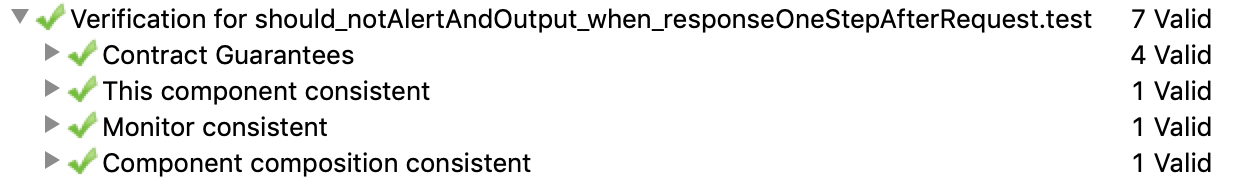
\includegraphics[scale=0.38]{agree-test-output.png} \\
    \end{tabular}
  \end{center}
  \caption{AGREE output for unit test.} 
  \label{fig:test-output}
\end{figure}